\documentclass[runningheads]{llncs}
\usepackage[T1]{fontenc}
\usepackage{graphicx}
\usepackage{booktabs}
\newcommand{\corr}{(*)}
% N.B.: do not change anything above this line. If you require additional packages, please load them directly after this line.
% \usepackage{mwe} % optional

% Add extra packages here (after the line above)
\usepackage{amsmath,amssymb} 
\usepackage{cleveref}
\usepackage{algorithm}
\usepackage{algpseudocode} 
\usepackage{tikz}
 
\IfFileExists{xcolor.sty}{\usepackage{xcolor}}{\usepackage{color}}
\definecolor{dpgCritical}{rgb}{1.000,0.851,0.400}      % #ffd966
\definecolor{dpgPredBranch}{rgb}{0.714,0.843,0.659}    % #b6d7a8
\definecolor{dpgCompBranch}{rgb}{0.957,0.800,0.800}    % #f4cccc
\definecolor{dpgFocus}{rgb}{0.624,0.773,0.910}         % #9fc5e8
\definecolor{dpgContext}{rgb}{0.973,0.976,0.984}       % #f8f9fb
\definecolor{dpgTrueLeaf}{rgb}{0.576,0.769,0.490}      % #93c47d
\definecolor{dpgOtherLeaf}{rgb}{0.902,0.722,0.686}

\usetikzlibrary{positioning,arrows.meta} 


\begin{document}

\title{Decision Predicate Graphs for Structurally Faithful Local Explanations of Tree Ensembles Beyond Output Agreement}

\titlerunning{DPGs for Faithful Local Explanations}

% For double-blind submission (recommended for initial review), use:
% \author{Author information scrubbed for double-blind reviewing}
% \authorrunning{Anonymous Authors}

% Camera-ready version (uncomment when not double-blind)
\author{Author information scrubbed for double-blind reviewing}
\authorrunning{Anonymous Authors}
\institute{}

\maketitle
\begin{abstract} %max 2000 chars
Output-level agreement is an insufficient criterion for local explanations when the goal is to diagnose how a model reached a specific decision, since two explanations can match a prediction equally well while differing substantially in path-level faithfulness. We address this through Decision Predicate Graphs (DPGs), extending the original global construction to DPG-local, which builds each explanation as a sample-specific subgraph from the exact root-to-leaf paths executed by the ensemble. On top of this structure, a Semantic Graph View provides three diagnostics: an explanation confidence score, competitor exposure quantifying support for the strongest alternative class, and a critical node identifying where predicted and competing paths last overlap before diverging. Across 15 benchmark datasets, near-complete trace recovery (edge recall $\approx$ 0.99) confirms structural faithfulness, while edge precision and zero recombination serve as construction-consistency checks. DPG-local remains competitive on shared output-level metrics against TreeSHAP, ICE, LIME, and Anchors, while providing structurally grounded diagnostics that output-aligned methods cannot offer.
\keywords{Explainable AI \and Local explanations \and Tree ensembles \and Random forests \and Decision Predicate Graphs \and Structural faithfulness}
\end{abstract}

\section{Introduction}
Explainable AI methods are commonly distinguished by the scope of the explanation they provide. Global explanations aim to characterise the behaviour of the predictive model as a whole, whereas local explanations are designed to explain a single prediction or the model's behaviour in the neighbourhood of a specific instance \cite{lundberg2020local,vilone2021notions,setzu2021glocalx}. Local explanations are especially important in decision-support settings because inspection, validation, contestability, and error analysis often arise at the level of an individual case rather than only at the level of aggregate model behaviour \cite{nauta2023anecdotal}.
Many widely used local explanation methods are optimised for \emph{prediction-level} faithfulness and express explanations primarily through \emph{input features} or feature conditions. Local Interpretable Model-agnostic Explanations (LIME), for instance, explain a prediction by fitting an interpretable surrogate in the neighbourhood of the query point, whereas Shapley Additive exPlanations (SHAP) decompose the prediction into additive feature contributions relative to a reference baseline \cite{ribeiro2016why,lundberg2017unified}. Related methods, such as Individual Conditional Expectation (ICE) and Anchors, likewise describe local behaviour through feature-wise sensitivity profiles or sufficient rule conditions \cite{goldstein2015ice,ribeiro2018anchors}. In Fr\"amling's terminology, these methods predominantly characterise \emph{feature influence}, that is, effects defined with respect to a baseline or perturbation distribution, rather than the broader notion of feature importance \cite{framling2023importanceinfluence}.
This perspective is useful, but insufficient for the problem targeted in this research. When the objective is to inspect how a model arrived at a specific inference, diagnose failure modes, or compare competing class hypotheses, fidelity -- understood as the degree to which an explanation accurately reflects its behaviour \cite{vilone2021notions} -- is too weak a criterion when only assessed at the final output level. Different local explanations may exhibit similar prediction-level fidelity but differ substantially in preserving the executed decision path and exposing the diagnostically relevant local decision structure.

\begin{figure}
    \centering
    \includegraphics[width=1\linewidth]{high-level-diagram.png}
    \caption{High-level diagram of the Decision Predicative Graphs complemented by the Semantic Graph View for structured local explanations}
    \label{fig:high-level-d}
\end{figure}

In this research article, we investigate the hypothesis that \emph{Decision Predicate Graphs} (DPG) can serve as a faithful and informative basis for local explanations of tree-ensemble predictions, because they encode a model inferential process directly at the level of standardised split predicates and their empirically observed transitions \cite{arrighi2024decision}. 
Accordingly, we represent each local explanation as a sample-specific sub-graph achieved by projecting the instance onto an obtained DPG. In this representation, nodes correspond to \emph{predicates} extracted from tree internal splits, that is, interpretable feature-value tests of the form $(x_j \leq \theta)$ (or $(x_j > \theta)$), where thresholds are mapped to a common vocabulary through rounding and consistent predicate formatting. 
Edges represent \emph{predicate transitions} activated along executed root-to-leaf paths, capturing the local ordering and co-occurrence of split conditions that lead to the predicted outcome.
Our central thesis is that local graph explanations should be evaluated not only by agreement with the model output, but also by how well they recover the executed decision structure and highlight where competing classes diverge. This matters because local explanations are often used to debug models, study errors, and compare alternative class hypotheses. In these settings, reproducing the predicted label is insufficient; the explanation must reflect the inferential route a model actually followed for the sample. Accordingly, we position DPG-local as a diagnostic layer for structural and contrastive analysis, rather than as a direct fidelity replacement for output-aligned methods such as TreeSHAP, as depicted in figure \ref{fig:high-level-d}. %https://docs.google.com/presentation/d/1BV8h52owXJUPlWYmvkfiRZtGHJDd8FI-ETV6AFVQ1NE/edit?usp=sharing
To enable DPG-based local explanations, we modify the graph construction used in the original DPG formulation and its extension \cite{arrighi2024decision,ceschin2025extending}. Instead of aggregating predicate transitions checking the training data, as the original version, we build each local graph from the exact root-to-leaf paths executed by the ensemble for the target sample. Aggregated transitions can splice together fragments that never appeared on the same tree path, yielding plausible labels but invalid local routes and weaker separation between the predicted and competing classes. Our DPG-local construction avoids this issue and allows the resulting local graph to be verified directly against the model's executed traces.

Besides the obtained DPG, we introduce a Semantic Graph View for structured local explanations. It reports (i) an \emph{explanation confidence score}, (ii) \emph{competitor exposure}, which quantifies how much support is assigned to the strongest alternative class, and (iii) a \emph{critical decision node}, defined as the last shared non-root predicate between the strongest predicted path and the strongest competitor path. 
These quantities are designed to go beyond aggregate benchmarking and to support disagreement-aware analysis and error diagnosis, in line with evidence that explanation disagreement is common in practice and requires explicit treatment \cite{krishna2022disagreement}. 
Moreover, by explicitly contrasting the predicted outcome with a competing alternative, this Semantic Graph View follows the broader view that explanations are often contrastive in nature \cite{miller2019explanation}. 
The contributions offered are:
\begin{itemize}
  \item a reformulation of DPG by building each explanation as a DPG-local graph extracted from the exact root-to-leaf paths activated by a tree ensemble on the inspected sample, and not from merged predicate-transition statistics.
  \item We distinguish DPG-local from tree-path summaries that also use executed paths: tree-path collapses evidence to feature-level rankings, whereas DPG-local preserves predicate-transition topology, branch competition, and critical decision gates as first-class local objects.
  \item We introduce a Semantic Graph View that summarises each DPG-local subgraph with class-contrastive, structure-aware descriptors, including an explanation confidence score, competitor exposure from the strongest alternative paths, and a critical decision node.
  \item We evaluate the method on 15 numeric tabular datasets against TreeSHAP, LIME, ICE, Anchors, and a tree-path baseline using shared metrics (output agreement with the model, confidence and margin behaviour, explanation size, and runtime) together with DPG-specific structural faithfulness metrics (predicate and transition recovery, and recombination rate).
\end{itemize}


% -----------------------------------------------------------------------
\section{Related Work}
% -----------------------------------------------------------------------

Local explanations for tabular predictors are often grouped into feature attribution, local-surrogate, response-profile, and rule-based  \cite{poeta2023concept}. This taxonomy mirrors the explanatory object returned by each method and its degree of alignment with an underlying model. It also reflects practical usage of explanations, where interpretability supports the communication of predictions and their debugging, auditing, and disagreement analysis in high-impact settings \cite{doshi2017rigorous,LONGO2024102301}.

\textit{Feature-attribution methods} explain predictions through per-feature contribution scores. TreeSHAP is the most established model-direct local explainer for tree ensembles and provides additive feature attributions with strong alignment to the model output under the SHAP axioms \cite{lundberg2017unified,lundberg2018consistent}. However, it represents an explanation as a vector of feature contributions and does not return an explicit local decision structure, so it does not support structural checks such as whether executed predicate transitions are preserved or whether predicted and competing classes share a decision gate.

\textit{Local surrogates and rule-based explainers} provide explanations through simplified models or sufficient conditions. LIME fits an interpretable surrogate in the neighbourhood of an instance \cite{ribeiro2016why}, and Anchors produces high-precision local rules \cite{ribeiro2018anchors}. Methods such as BELLATREX and RuleFit operate over tree-derived predicates, but return rule sets or surrogate rule models rather than a local graph object whose transitions can be validated against executed traces \cite{dedja2023bellatrex,friedman2008predictive}. BELLATREX is closer to DPG-local in being model-direct and tree-derived, but it returns a selected rule set rather than an ordered predicate-transition graph, so it does not preserve full transition ordering as a first-class output and provides no recombination diagnostic. The same applies to RuleFit.

\textit{Response-profile methods} focus on what-if behavior. ICE plots vary a single feature while keeping others fixed \cite{goldstein2015ice}, which is valuable as a sensitivity diagnostic but does not represent the route taken by a tree ensemble for a specific instance. We also include a tree-path baseline \cite{palczewska2014interpreting} that follows executed forest paths but reduces structure to per-feature scores, discarding path transitions and predicted-versus-competitor branch competition.

Our \textit{Semantic Graph View} is motivated by two recurring observations: explanations are often contrastive \cite{miller2019explanation,van2021evaluating,LongoRizzo2024}, and different explainers can disagree substantially for the same model and input \cite{krishna2022disagreement}.
 These observations motivate reporting competitor exposure and explicit predicted-versus-competitor comparisons, rather than only a single-class summary.
 

 Recent evaluation work further emphasises that output-level fidelity alone is insufficient and that faithfulness should be assessed through complementary criteria \cite{nauta2023anecdotal,doshi2017rigorous}. In line with this view, we evaluate all methods using shared metrics where applicable and complement them with structural measures that are meaningful only for DPG-local graphs. 

Table~\ref{tab:positioning} summarises the main baselines. ``Partial'' structural faithfulness ($\sim$) means a method uses tree-derived predicates or path fragments but does not return a local graph with ordered predicate transitions that can be validated edge by edge against executed traces; ``Supported'' ($\checkmark$) requires (i) explicit transition ordering, (ii) branch/topology preservation, and (iii) direct trace-level structural checks (edge recall/precision and recombination diagnostics).


\begin{table}[h!]
\centering
\caption{Positioning of local explanation methods. Faith.\ denotes structural faithfulness checks against executed traces; Contrast denotes explicit predicted-vs-competitor diagnostics. Access: \texttt{d}=model-direct, \texttt{a}=model-agnostic.}
\label{tab:positioning}
\small
\setlength{\tabcolsep}{6pt}
\begin{tabular}{l l c c c}
\hline
Method & Object & Access & Faith. & Contrast \\
\hline
TreeSHAP \cite{lundberg2018consistent} & feature attributions & \texttt{d} & $\times$ & $\sim$ \\
LIME \cite{ribeiro2016why} & local surrogate & \texttt{a} & $\times$ & $\sim$ \\
ICE \cite{goldstein2015ice} & response profile & \texttt{a} & $\times$ & $\times$ \\
Anchors \cite{ribeiro2018anchors} & rule conditions & \texttt{a} & $\times$ & $\sim$ \\
BELLATREX \cite{dedja2023bellatrex} & diverse rule set & \texttt{d} & $\sim$ & $\sim$ \\
RuleFit / rule ens. \cite{friedman2008predictive} & rule model / rule set & \texttt{d} & $\sim$ & $\sim$ \\
Tree-path \cite{palczewska2014interpreting} & path-based ranking & \texttt{d} & $\sim$ & $\times$ \\
\hline
DPG-local (ours) & DPG-local graph & \texttt{d} & $\checkmark$ & $\checkmark$ \\
\hline
\end{tabular}
\end{table}

% -----------------------------------------------------------------------
\section{Method}
% -----------------------------------------------------------------------

%\subsection{DPG and the Local-Explanation Gap}

Decision Predicate Graphs (DPGs) represent tree ensembles as directed graphs: nodes are standardised split predicates and edges observed predicate transitions \cite{arrighi2024decision,ceschin2025extending}..  While DPGs enable the extraction of graph metrics for model inspection such formulation is \emph{global}: transitions are aggregated across all training samples, thus traversing the global graph for a single instance can stitch together edge fragments from other samples or different trees that were never jointly executed for that instance -- we refer to this as \emph{recombination}. Unfortunately, this mitigates local faithfulness when the explanation target is the exact executed decision process and not the final predicted label. Our goal is to leverage on the DPG;s data structure but replacing its local construction rule: local graphs must be built from exact sample-specific execution traces, not from global transition statistics.

\subsection{DPG-local Construction}
\label{sec:dpg-construction}

Let $\mathcal{F}=\{T_b\}_{b=1}^B$ be a trained tree ensemble with $B$ baselearners. For a sample $x$, let $\pi_b(x)=[p^{(b)}_1,\dots,p^{(b)}_{L_b}]$ be the executed root-to-leaf predicate sequence in baselearner $T_b$, where $L_b$ is its path length. Predicates are standardised with a deterministic map $\phi(\cdot)$ (feature naming plus threshold rounding).
The DPG-local version builds $G_x$ using only the transitions executed for the inspected sample $x$, containing sample-specific realised transitions rather than globally valid but potentially non-co-occurring fragments. Constructing one local graph costs $O(BL_x)$, removing dependence on a separate global-graph traversal stage. The decision predicate graph is $G_x=(V_x,E_x,\omega_x)$:
\begin{itemize}
  \item $V_x$: set of standardised predicate nodes reached for sample $x$;
  \item $E_x$: set of directed transitions of consecutive predicates in executed paths;
  \item $\omega_x(e)$: normalized support of edge $e$, computed as its frequency across the $B$ baselearners.
\end{itemize}

Hence, every edge in $G_x$ is backed by at least one executed trace for $x$. Node support separates stable conditions from incidental ones, edge support makes dominant and weak local routes explicit, class-terminal support exposes predicted-versus-competitor evidence and branching concentration clarifies if the local decision is decisive or contested (full pseudocode in Algorithm~\ref{alg:exec-trace-dpg}), with per-sample cost $O(\sum_{b=1}^{B}L_b)$ and memory $O(|V_x|+|E_x|)$.
Because the main rationale of DPG-local is to avoid stitching non-jointly executed transitions, we track recombination directly. 
With $\Gamma_x=E_x^{edge}\setminus T_x^{edge}$, recombination rate is:
$$ \mathrm{RecombinationRate}_x=\frac{|\Gamma_x|}{|E_x^{edge}|+\varepsilon}.$$
Lower values indicate fewer non-executed transition fragments in the local graph (example of DPG-local graph in Fig.~\ref{fig:dpg-example}).

\begin{algorithm}[ht]
\caption{DPG-local construction}
\label{alg:exec-trace-dpg}
\begin{algorithmic}[1]
\Require sample $x$, tree ensemble $\mathcal{F}=\{T_b\}_{b=1}^B$, standardization map $\phi$
\Ensure local graph $G_x=(V_x,E_x,\omega_x)$
\State $V_x \gets \emptyset$, $E_x \gets \emptyset$
\State $c_e \gets$ empty map from edges to counts
\For{$b=1$ to $B$}
  \State $\pi_b(x) \gets$ executed root-to-leaf predicate sequence in $T_b$
  \State $\hat{\pi}_b(x) \gets [\phi(p)\ \text{for}\ p\in\pi_b(x)]$
  \State add all predicates in $\hat{\pi}_b(x)$ to $V_x$
  \For{each consecutive pair $(u,v)$ in $\hat{\pi}_b(x)$}
    \State add $(u,v)$ to $E_x$;\quad $c_e[(u,v)] \gets c_e[(u,v)] + 1$
  \EndFor
\EndFor
\For{each edge $e\in E_x$}
  \State $\omega_x(e) \gets c_e[e]/B$
\EndFor
\State \Return $G_x=(V_x,E_x,\omega_x)$
\end{algorithmic}
\end{algorithm}

\begin{figure}[ht]
\centering
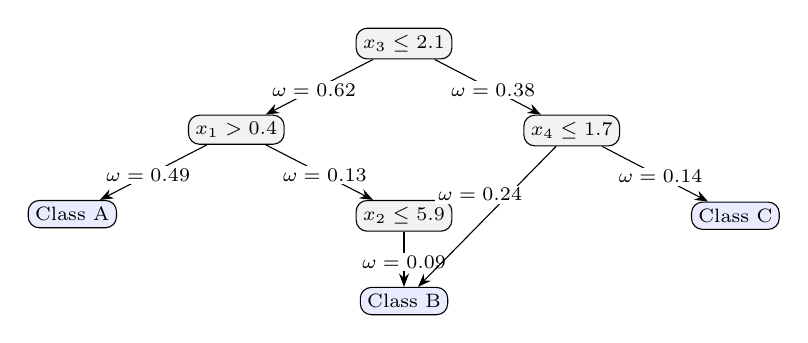
\begin{tikzpicture}[
  >=Stealth,
  node distance=7mm and 9mm,
  pred/.style={rectangle, rounded corners, draw=black, fill=gray!10, align=center, font=\scriptsize, inner sep=2.5pt},
  cls/.style={rectangle, rounded corners, draw=black, fill=blue!8, align=center, font=\scriptsize, inner sep=2.5pt},
  elab/.style={font=\scriptsize, fill=white, inner sep=1pt}
]
\node[pred] (p1) {$x_3 \le 2.1$};
\node[pred, below left=of p1] (p2) {$x_1 > 0.4$};
\node[pred, below right=of p1] (p3) {$x_4 \le 1.7$};
\node[pred, below right=of p2] (p4) {$x_2 \le 5.9$};
\node[cls, below left=of p2] (cA) {Class A};
\node[cls, below=of p4] (cB) {Class B};
\node[cls, below right=of p3] (cC) {Class C};
\draw[->] (p1) -- node[elab, pos=0.55] {$\omega=0.62$} (p2);
\draw[->] (p1) -- node[elab, pos=0.55] {$\omega=0.38$} (p3);
\draw[->] (p2) -- node[elab, pos=0.55] {$\omega=0.49$} (cA);
\draw[->] (p2) -- node[elab, pos=0.55] {$\omega=0.13$} (p4);
\draw[->] (p4) -- node[elab, pos=0.55] {$\omega=0.09$} (cB);
\draw[->] (p3) -- node[elab, pos=0.55, above, yshift=7pt] {$\omega=0.24$} (cB);
\draw[->] (p3) -- node[elab, pos=0.55] {$\omega=0.14$} (cC);
\end{tikzpicture}
\caption{Illustrative DPG-local graph for one sample. Rectangles are standardised predicate nodes, rounded blue rectangles are class terminals, and edge labels are normalised transition support.}
\label{fig:dpg-example}
\end{figure}




\subsection{Semantic Graph View} \label{sec:semantic-layer}
The DPG-local construction gives a trace-faithful local graph, but diagnosis requires compact quantities comparable across samples and datasets. We derive metrics targeting three needs: separation between predicted and competing classes, concentration of evidence, and agreement between the explanation and the ensemble decision. The confidence score aggregates these signals under structural coverage, so high confidence is reported only when both semantic support and trace recovery are strong.
From $G_x$, we extract weighted explanation paths $\mathcal{P}_x=\{(p,w_x(p),y(p))\}$, where $p$ is a local path, $w_x(p)\ge 0$ is its support, and $y(p)$ is its class endpoint. We normalize supports as $\tilde{w}_x(p)={w_x(p)}/{\sum_{q\in\mathcal{P}_x} w_x(q)+\varepsilon}$ with $\varepsilon=10^{-12}$. Class support $S_x(y)$ sums normalised path support over all paths ending in class $y$. The explanation class $\hat{y}^{exp}_x$ has largest support; the strongest competitor $y_x^{(2)}$ has highest remaining support.
The \emph{margin} $M_x=S_x(\hat{y}^{exp}_x)-S_x(y_x^{(2)})$ measures class separation. \emph{Path purity} $\mathrm{PathPurity}_x=S_x(\hat{y}^{exp}_x)$ and \emph{competitor exposure} $\mathrm{CompetitorExposure}_x=1-\mathrm{PathPurity}_x$ quantify support concentration.
\emph{Top-$K$ concentration} $C_x^{(K)}$ (with $K=3$) captures whether predicted-class evidence is dominated by a few paths. \emph{Vote agreement} $A_x=V_x(\hat{y}^{exp}_x)/B$ quantifies alignment with the ensemble vote, where $V_x(y)$ is the number of baselearners voting for class $y$. \emph{Structural coverage} $G_x^{cov}=(R_x^{node}+R_x^{edge})/2$ summarizes trace recovery.
These are combined into the \emph{explanation confidence}:
\[
\mathrm{Conf}_x=G_x^{cov}\cdot\frac{M_x+C_x^{(K)}+A_x}{3}.
\]
The combination is scale-consistent: all four components lie in $[0,1]$, so $\mathrm{Conf}_x\in[0,1]$.
An unweighted mean of $(M_x,C_x^{(K)},A_x)$ avoids dataset-specific tuning.


\begin{table}[h!]
\centering
\small
\caption{Semantic Graph View metrics and their explainability use.}
\label{tab:semantic-metrics}
\setlength{\tabcolsep}{5pt}
\begin{tabular}{p{3.3cm} p{8.5cm}}
\toprule
Metric & Explainability use \\
\midrule
Class support & Quantifies evidence assigned to each class from local paths. \\
\addlinespace[1pt]
Predicted/ competitor class & Identifies the explained outcome and the strongest alternative for contrastive analysis. \\
\addlinespace[1pt]
Margin & Measures separation of predicted and competitor classes. \\
\addlinespace[1pt]
Path purity & Indicates how much support remains on the predicted class. \\
\addlinespace[1pt]
Competitor exposure & Indicates how much support shifts toward alternative classes. \\
\addlinespace[1pt]
Top-$K$ concentration & Shows evidence concentration of a few dominant paths. \\
\addlinespace[1pt]
Vote agreement & Checks alignment between the explanation class and the ensemble voting behaviour. \\
\addlinespace[1pt]
Structural coverage & Summarises node/edge recovery of executed traces. \\
\addlinespace[1pt]
Explanation confidence & synthesises a single structure of local explanation quality. \\
\bottomrule
\end{tabular}
\end{table}

Its coverage acts as a multiplicative reliability gate that down-weights strong semantic signals when trace recovery is weak.
This is not a probability-calibration measure but a compact summary of structural coverage, class separation, evidence concentration, and ensemble agreement. Table~\ref{tab:semantic-metrics} summarises all Semantic Graph View metrics and their explainability use.






\subsection{Critical Node and Structural Faithfulness}
\label{sec:structural-faithfulness}

We use the strongest predicted-class path $p_x^\ast$ and the strongest competitor path $q_x^\ast$ to localise where the explanation route diverges. Comparing the two ordered node sequences through their longest common prefix, the last shared non-root predicate is the \emph{critical node} $c_x$ at depth $d_x$. Branch contrast $\Delta_x^{crit}=|B_x(s_x^{pred})-B_x(s_x^{comp})|$ measures post-split support divergence, where $B_x(\cdot)$ is normalized branch support after the critical split (Figure~\ref{fig:critical-node-example}). This localisation supports contrastive reasoning, targeted what-if analysis, and error diagnosis by characterising whether divergence is early, late, sharp, or weak.

\textit{Structural faithfulness} is evaluated with specifically for executed traces. Let $(T_x^{node},T_x^{edge})$ be trace node/edge sets and $(E_x^{node},E_x^{edge})$ the explanation sets. Node and edge recall/precision are intersection-over-trace-size and intersection-over-explanation-size, respectively ($\varepsilon=10^{-12}$ smoothing in denominators), complemented by recombination rate from Section~3.2.

\begin{figure}[h]
\centering
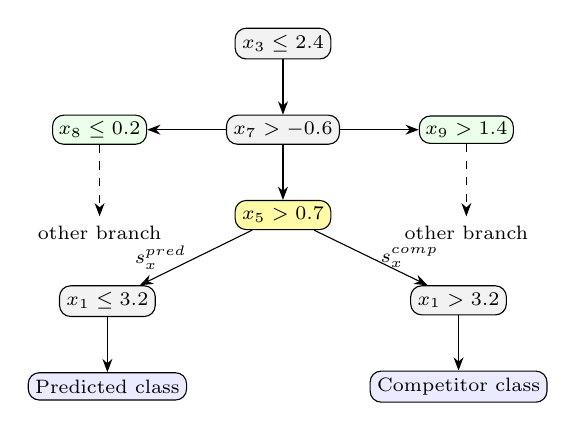
\begin{tikzpicture}[
  >=Stealth,
  node distance=7.0mm and 10.0mm,
  pred/.style={rectangle, rounded corners, draw=black, fill=gray!10, align=center, font=\scriptsize, inner sep=2.5pt},
  crit/.style={rectangle, rounded corners, draw=black, fill=yellow!35, align=center, font=\scriptsize, inner sep=2.5pt},
  cls/.style={rectangle, rounded corners, draw=black, fill=blue!8, align=center, font=\scriptsize, inner sep=2.5pt},
  side/.style={rectangle, rounded corners, draw=black, fill=green!8, align=center, font=\scriptsize, inner sep=2.2pt}
]
\node[pred] (p1) {$x_3 \le 2.4$};
\node[pred, below=of p1] (p2) {$x_7 > -0.6$};
\node[crit, below=of p2] (c) {$x_5 > 0.7$};
\node[pred, below left=of c] (pp1) {$x_1 \le 3.2$};
\node[cls, below=of pp1] (yp) {Predicted class};
\node[pred, below right=of c] (pc1) {$x_1 > 3.2$};
\node[cls, below=of pc1] (yc) {Competitor class};
\node[side, left=of p2] (s1) {$x_8 \le 0.2$};
\node[side, right=of p2] (s2) {$x_9 > 1.4$};
\draw[->] (p1) -- (p2);
\draw[->] (p2) -- (c);
\draw[->] (p2) -- (s1);
\draw[->] (p2) -- (s2);
\draw[->] (c) -- node[font=\scriptsize, left] {$s_x^{pred}$} (pp1);
\draw[->] (c) -- node[font=\scriptsize, right] {$s_x^{comp}$} (pc1);
\draw[->] (pp1) -- (yp);
\draw[->] (pc1) -- (yc);
\draw[dashed,->] (s1) -- ++(0,-1.1) node[below,font=\scriptsize] {other branch};
\draw[dashed,->] (s2) -- ++(0,-1.1) node[below,font=\scriptsize] {other branch};
\end{tikzpicture}
\caption{Illustration of Critical-node: two strongest paths share prefix $x_3 \le 2.4 \to x_7 > -0.6 \to$ critical node, but diverge in predicted and competitor successors. Side branches show that alternative paths, not part of the two strongest,  coexist in the local graph.}
\label{fig:critical-node-example}
\end{figure}

% -----------------------------------------------------------------------
\section{Experimental Setup}
% -----------------------------------------------------------------------

\subsection{Datasets and Models}
We evaluate our method on 15 numeric tabular  datasets for classification tasks: \texttt{banknote-authentication}, \texttt{breast\_cancer}, \texttt{diabetes}, \texttt{digits}, \texttt{ionosphere}, \texttt{iris}, \texttt{isolet}, \texttt{madelon}, \texttt{phoneme}, \texttt{qsar-biodeg}, \texttt{segment}, \texttt{spambase}, \texttt{vehicle}, \texttt{wdbc}, and \texttt{wine} (Table~\ref{tab:datasets-models-summary}). These cover binary and multiclass tasks with very different feature counts and levels of predicate reuse, important for evaluating structural faithfulness on both simple and harder ensemble decision boundaries.
For every dataset we train random forest classifiers with search space $n_{\mathrm{estimators}} \in \{10,20\}$, $\mathrm{max\_depth}=4$, $\mathrm{perc\_var} \in \{10^{-4},10^{-5}\}$, and $\mathrm{decimal\_threshold}=6$, where $\mathrm{perc\_var}$ is the minimum path-frequency ratio used to keep predicate transitions in the DPG construction pipeline, and $\mathrm{decimal\_threshold}$ is the number of decimal digits used to round split thresholds when predicates are standardized. Each configuration is repeated with seeds $27$ and $42$. The best DPG-local configuration per dataset is selected by ranking runs on local match rate ($\mathrm{local\_matches\_model\_rate}$, the fraction of samples where the explanation class equals the model-predicted class), edge precision, node precision, recombination rate, and explanation confidence, in that order.


\begin{table}[t]
  \centering
  \small
  \caption{Dataset and model summary. `Avg.\ RF Perf.' is averaged across configurations and seeds.}
  \label{tab:datasets-models-summary}
  \begin{tabular}{lcccc}
    \toprule
    Dataset & \#Classes & \#Features & \#Samples & Avg. RF Perf. \\
    \midrule
    banknote-authentication & 2 & 4 & 1372 & 0.963 \\
    breast\_cancer & 2 & 30 & 569 & 0.950 \\
    diabetes & 2 & 8 & 768 & 0.726 \\
    digits & 10 & 64 & 1797 & 0.848 \\
    ionosphere & 2 & 34 & 351 & 0.939 \\
    iris & 3 & 4 & 150 & 0.944 \\
    isolet & 26 & 617 & 7797 & 0.714 \\
    madelon & 2 & 500 & 2600 & 0.626 \\
    phoneme & 2 & 5 & 5404 & 0.818 \\
    qsar-biodeg & 2 & 41 & 1055 & 0.816 \\
    segment & 7 & 19 & 2310 & 0.850 \\
    spambase & 2 & 57 & 4601 & 0.906 \\
    vehicle & 4 & 18 & 846 & 0.695 \\
    wdbc & 2 & 30 & 569 & 0.956 \\
    wine & 3 & 13 & 178 & 0.987 \\
    \bottomrule
  \end{tabular}
\end{table}


\subsection{Compared Methods, Metrics and statistical analysis}
The comparison includes DPG-local, DPG-global, and five baselines: TreeSHAP, LIME, ICE, Anchors, and a tree-path baseline aggregating class-probability changes along executed tree paths. This mix covers model-direct and local-surrogate families. TreeSHAP, tree-path, and Anchors are evaluated on the trained random forest directly; LIME provides the local-surrogate reference point.
Baseline hyperparameters: TreeSHAP uses 200 background instances; LIME uses 20 explanation features and 1000 perturbed samples; ICE uses 21 grid points; Anchors uses precision target $0.95$, maximum rule length 4, and at most 12 candidate conditions per expansion step.
We report \emph{fidelity} (fraction where explained class matches model prediction), \emph{local accuracy} (fraction where explained class matches ground-truth label), and \emph{margin} (difference between top explained class score and strongest competitor score) \cite{vilone2021notions,nauta2023anecdotal,doshi2017rigorous,miller2019explanation}; \emph{sufficiency}  which keeps only the explanation-selected features (replacing others with a training-set reference) and measures target-class probability; and \emph{comprehensiveness} \cite{nauta2023anecdotal} which removes selected features and measures the probability drop. The semantic-faithfulness protocol allocates the same feature budget to all methods.

\subsubsection{DPG-local-Specific Metrics.}
Beyond shared metrics, only DPG-local is evaluated on node/edge recall\slash precision, recombination rate, explanation confidence, critical-node metrics (split depth, branch contrast), disagreement-aware cohort summaries, and critical-branch intervention metrics. The cohort analysis separates model-correct/explanation-correct (MC-EC), model-wrong/explanation-matches-model (MW-EM), and disagreement cases. The critical-branch analysis is only for samples with a non-root critical node, measuring the shifts of model' probability to the competitor branch after intervening at the critical split.

\subsubsection{Statistical Analysis}
Results are reported at the dataset level; aggregation across datasets is performed after per-dataset best-configuration selection. We use the Friedman test for global method differences and paired Wilcoxon signed-rank tests for DPG-local vs.\ each baseline.


% -----------------------------------------------------------------------
\section{Results}
% -----------------------------------------------------------------------
\begin{figure}[ht!]
  \centering
  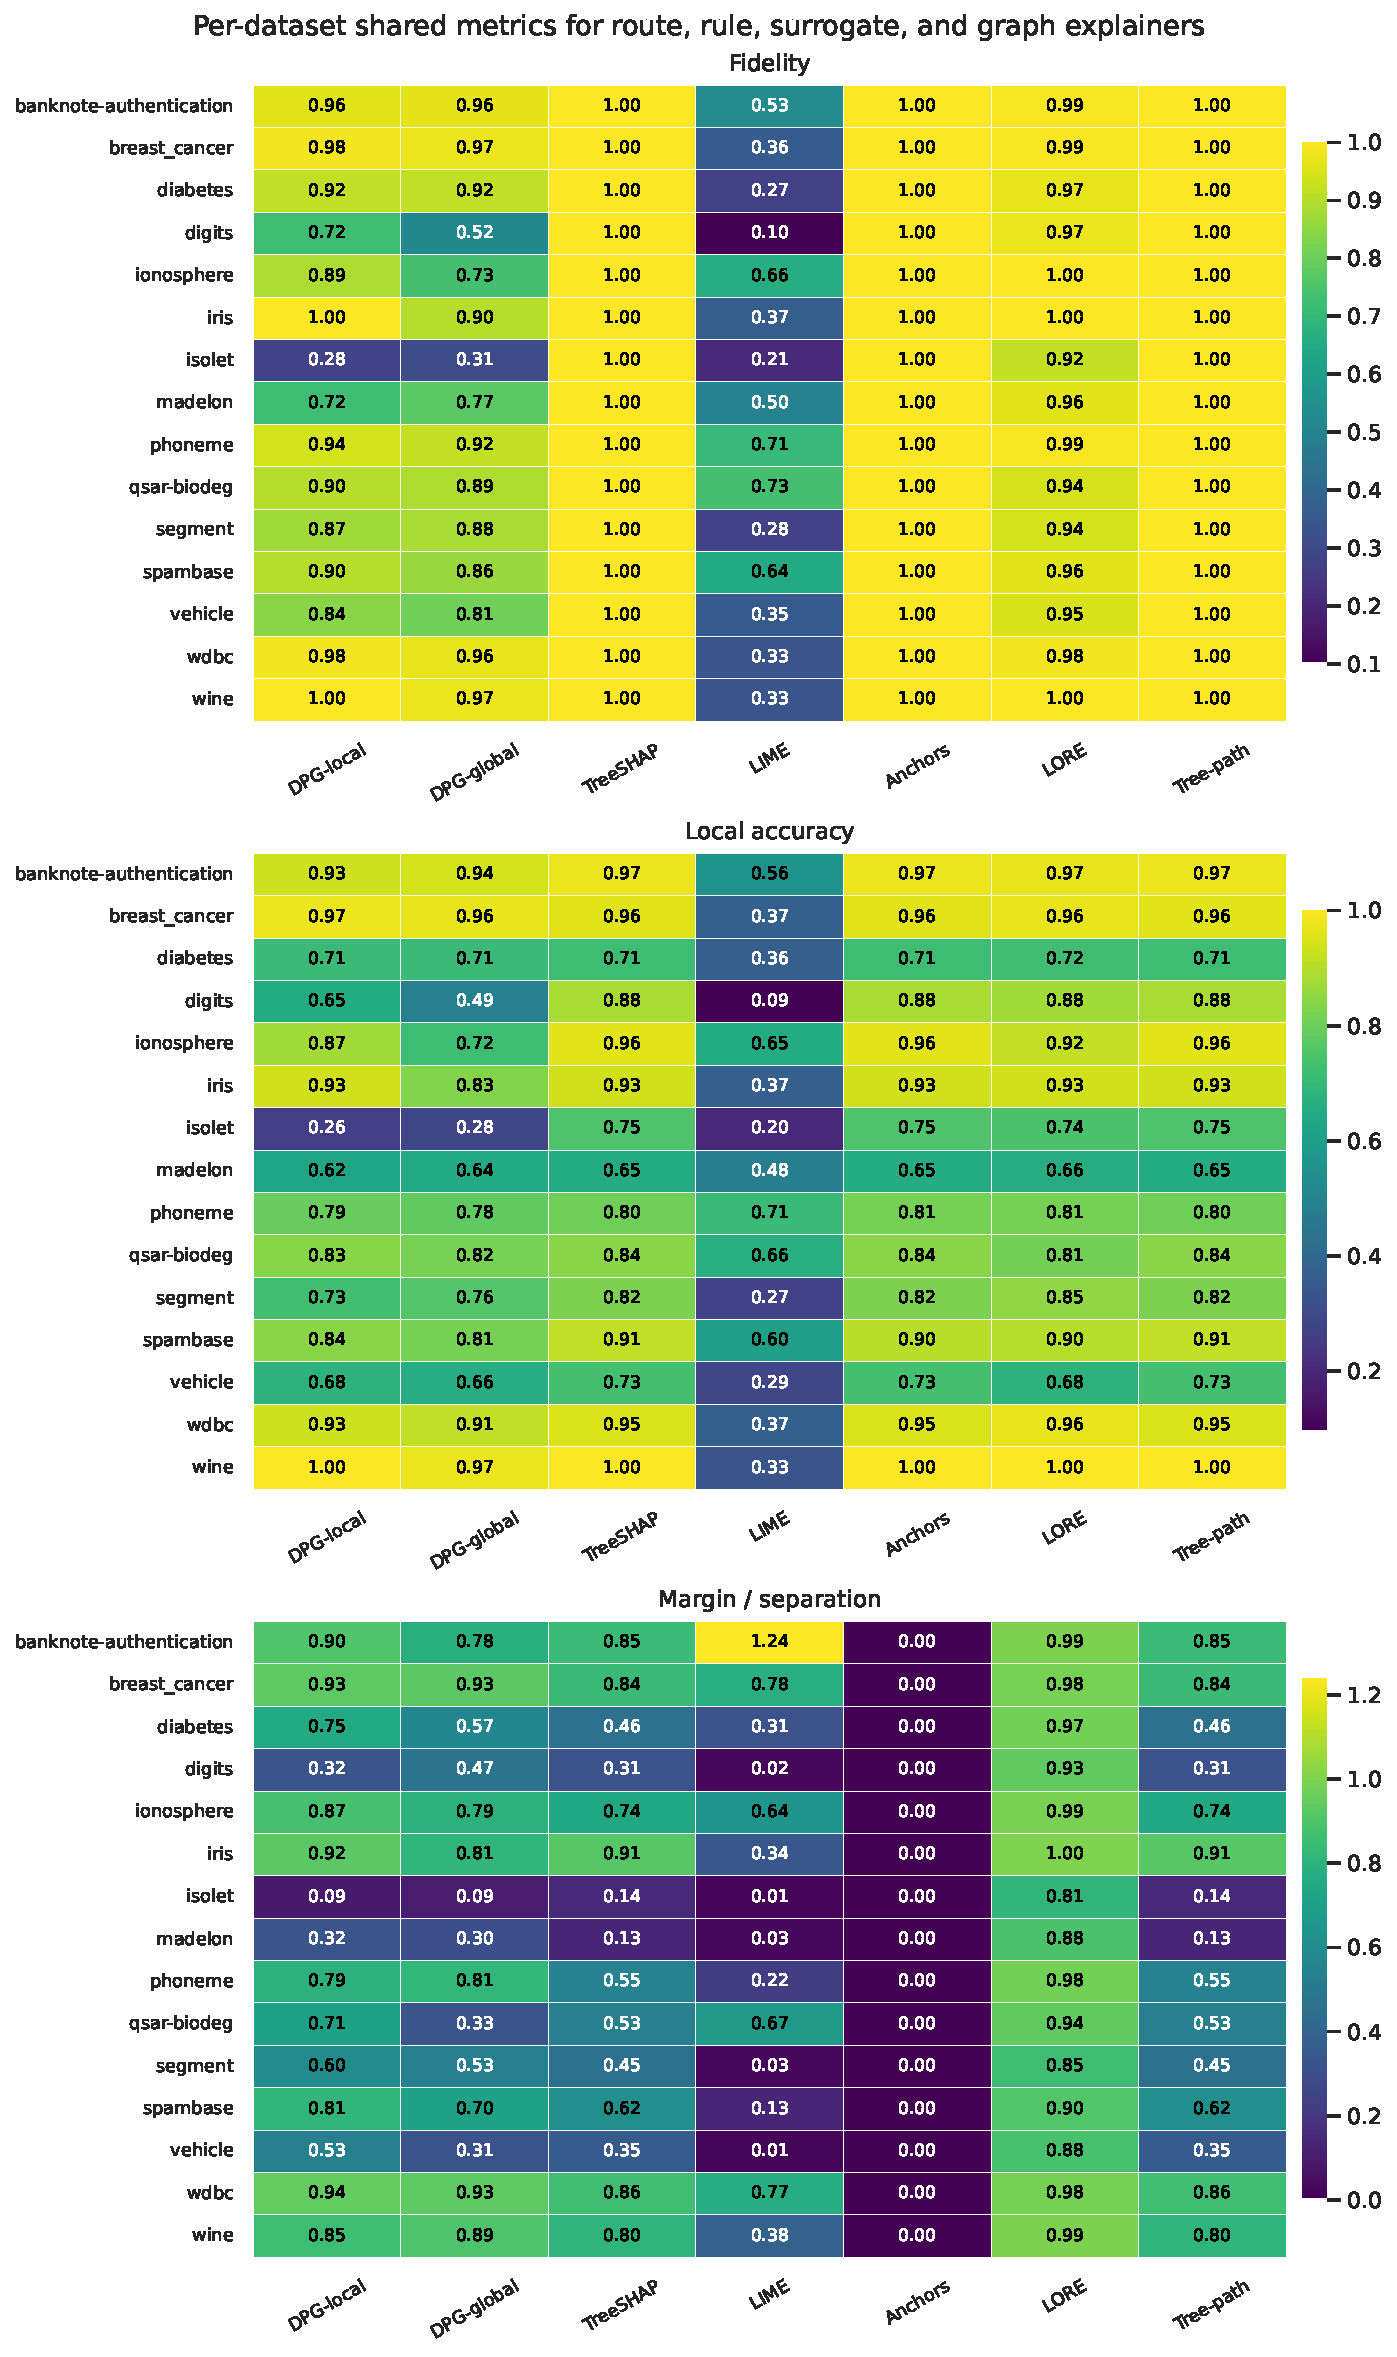
\includegraphics[width=\textwidth,height=1\textheight,keepaspectratio]{per_dataset_shared_metrics_heatmap.pdf}
  \caption{Per-dataset shared metrics as heatmaps. Rows are datasets, columns are methods (including DPG-local and DPG-global); darker cells indicate higher values.}
  \label{fig:per-dataset-results}
\end{figure}

\subsection{Baseline Comparison on Shared Metrics}
The results in Figure~\ref{fig:per-dataset-results} compare optimisation targets, not a single ranking. TreeSHAP, Tree-path, and Anchors dominate fidelity and local accuracy because they are explicitly designed to preserve model predictions. DPG-local is optimised for structural faithfulness (a surrogate representation), so lower fidelity relative to output-aligned baselines is expected. On margin, Anchors scores near zero because it returns a sufficient predicted-class rule without graded competitor decomposition, whereas DPG-local dominates ICE and LIME by explicitly modelling predicted-versus-competitor path support.



The Friedman test rejects equal performance across datasets ($p < 10^{-6}$ for all three metrics). Paired Wilcoxon tests show DPG-local is significantly below TreeSHAP on fidelity ($p=0.0015$) and local accuracy ($p=0.0012$), and below tree-path on fidelity ($p=0.0015$) and local accuracy ($p=0.0079$). On margin, DPG-local is not significantly different from TreeSHAP ($p=0.454$, higher on 10/15 datasets) but significantly exceeds tree-path ($p<10^{-4}$), ICE ($p=0.0020$), LIME ($p<10^{-4}$), and Anchors ($p<10^{-4}$). The Friedman statistic for margin is $\chi^2(5)=61.47$, $p=6.04\times 10^{-12}$.

The controlled internal ablation between DPG-global and DPG-local directly supports the main design claim. Across 15 datasets, DPG-local improves mean fidelity from $0.88$ to $0.90$, mean local accuracy from $0.79$ to $0.80$, and mean margin from $0.63$ to $0.73$, with dataset-level wins of 8/15, 8/15, and 11/15, respectively. Edge precision and zero recombination are consistent with the trace-restricted construction and act as sanity checks; the key empirical gain is in margin and structural fidelity. DPG-local should therefore be interpreted as complementary to TreeSHAP and tree-path: it adds a structure-aware diagnostic view (branch topology, competitor exposure, critical nodes) rather than targeting the same objective as output-fidelity explainers.

\subsection{Semantic Faithfulness}

This subsection focuses on DPG-local, LIME, and ICE because they are directly
comparable under the same perturbation-based, matched feature-budget protocol. Here, the comprehensiveness drop denotes the decrease in the predicted class
probability after removing the features selected by the explanation; higher
values indicate that the selected subset captures features on which the model
more strongly relies. Under this subgroup protocol, DPG-local reaches a mean
sufficiency probability of $0.54$ and a mean comprehensiveness drop of $0.13$,
close to LIME ($0.55$ and $0.17$) and above ICE in comprehensiveness
($0.07$) (table \ref{tab:semantic-faithfulness}).


\subsection{Structural Faithfulness, Disagreement, and Misclassification}

Structural metrics are the dimension in which DPG-local construction provides its main advantage. Since there is no directly comparable graph-based baseline in our setting, this subsection reports a DPG-local-centred structural evaluation across datasets. Across all evaluated datasets, DPG-local explanations contain on average $17.30$ active paths and $57.50$ active nodes per sample, while preserving the executed model structure almost exactly: mean edge precision is $1.00$, mean edge recall is $1.00$, and mean recombination is $0.00$ (Table~\ref{tab:dpg-structural}). Under DPG-local construction, edge precision and recombination are expected near-deterministic consistency checks (only executed edges are inserted), so the key empirical structural result is the near-complete edge recall ($\approx0.99$), which confirms that the constructed local graph retains almost all executed transitions in practice.


\begin{table}[ht!]
  \centering
  \small
  \caption{Semantic-faithfulness comparison for the focused subgroup
    (DPG-local, LIME, ICE) under the matched feature-budget protocol. Higher
    sufficiency probability and comprehensiveness drop are better.
    The critical-flip rate is defined only for DPG-local samples with a valid
    non-root
    critical node and is reported as a pooled global rate across all evaluated
    benchmark samples.}
  \label{tab:semantic-faithfulness}
  \begin{tabular}{lccc}
    \toprule
    Method                    & Sufficiency Prob. & Comprehensiveness Drop &
    Critical Flip Rate
    \\
    \midrule
    DPG-local & 0.54             & 0.13                  &
    <0.01
    \\
    LIME                      & 0.55             & 0.17                  & --
    \\
    ICE                       & 0.48             & 0.07                  & --
    \\
    \bottomrule
  \end{tabular}
\end{table}

\begin{table}[ht!]
\centering
\small
\caption{DPG-local structural and semantic diagnostics. Edge precision/recombination are construction-consistency checks; edge recall and cohort/disagreement shifts are the main empirical diagnostics.}
\label{tab:dpg-structural}
\begin{tabular}{lcccccc}
\toprule
Group & Conf. & Margin & Purity & Comp. Exp. & Edge Prec. & Recomb. \\
\midrule
Overall  & 0.69 & 0.73 & --   & --   & 1.00 & 0.00 \\
Agree    & 0.70 & 0.75 & --   & --   & --   & 0.00 \\
Disagree & 0.48 & 0.23 & --   & --   & --   & 0.00 \\
MC-EC    & 0.71 & --   & 0.87 & 0.13 & 1.00 & 0.00 \\
MW-EM    & 0.63 & --   & 0.77 & 0.24 & 1.00 & 0.00 \\
\bottomrule
\end{tabular}
\end{table}

Mean explanation confidence is $0.69$, ranging from $0.42$ (\texttt{isolet}) to $0.82$ (\texttt{ionosphere}), reflecting dataset difficulty. The dominant cohort is MC-EC (mean rate $0.79$), with confidence $0.71$, path purity $0.87$, and competitor exposure $0.13$. Model-wrong explanations (MW-EM) remain relatively confident ($0.63$, purity $0.77$), showing that a structurally coherent explanation can still support the wrong class when the ensemble itself is wrong.
The disagreement split is the most informative result. Agreement cases show confidence $0.70$, margin $0.75$, and model-vote agreement $0.84$; disagreement cases drop to $0.48$, $0.23$, and $0.38$ respectively, despite near-perfect trace coverage in both groups. Effect sizes are large: Cohen's $d=-1.97$ for confidence, $d=-1.86$ for margin, $d=-2.97$ for vote agreement, and $d=2.18$ for competitor exposure ($0.61$ vs.\ $0.18$). Disagreement is thus not random noise but a measurable redistribution of support toward competing branches.
The critical-branch intervention applies only when predicted and competitor paths share a non-root prefix. In \texttt{vehicle}, eight samples admit a non-root critical node and the intervention flips toward the competitor branch in $37.5\%$ of those cases --- a conditional rate over the eight valid cases, not contradicting the near-zero pooled rate in Table~\ref{tab:semantic-faithfulness} which covers all samples regardless of eligibility.

\subsection{Case Study}
The qualitative analysis uses local-subgraph analysis that preserves readability while retaining enough context to inspect critical nodes, successor branches, and alternative class endpoints. \Cref{fig:phase-cases} reports one DPG-local example, \texttt{vehicle} sample $56$. In this DPG-local structure,  \texttt{MAX.LENGTH\_ASPECT\_RATIO>-0.231807} (yellow) is the critical node. The two highlighted successors from that node lead to different outcomes: the red branch moves toward class $1$ (model prediction), whereas the green branch toward class $2$ (competitor/true class). Their close support, reflected by the small support margin ($0.04$), indicates a locally ambiguous decision in which a small structural shift after the critical split is sufficient to favour the competitor branch. This makes the sample a recovery/disagreement case and shows the diagnostic role of the critical node: it isolates the specific local gate where predicted-versus-competitor evidence diverges.

\begin{figure}[bt!]
\centering
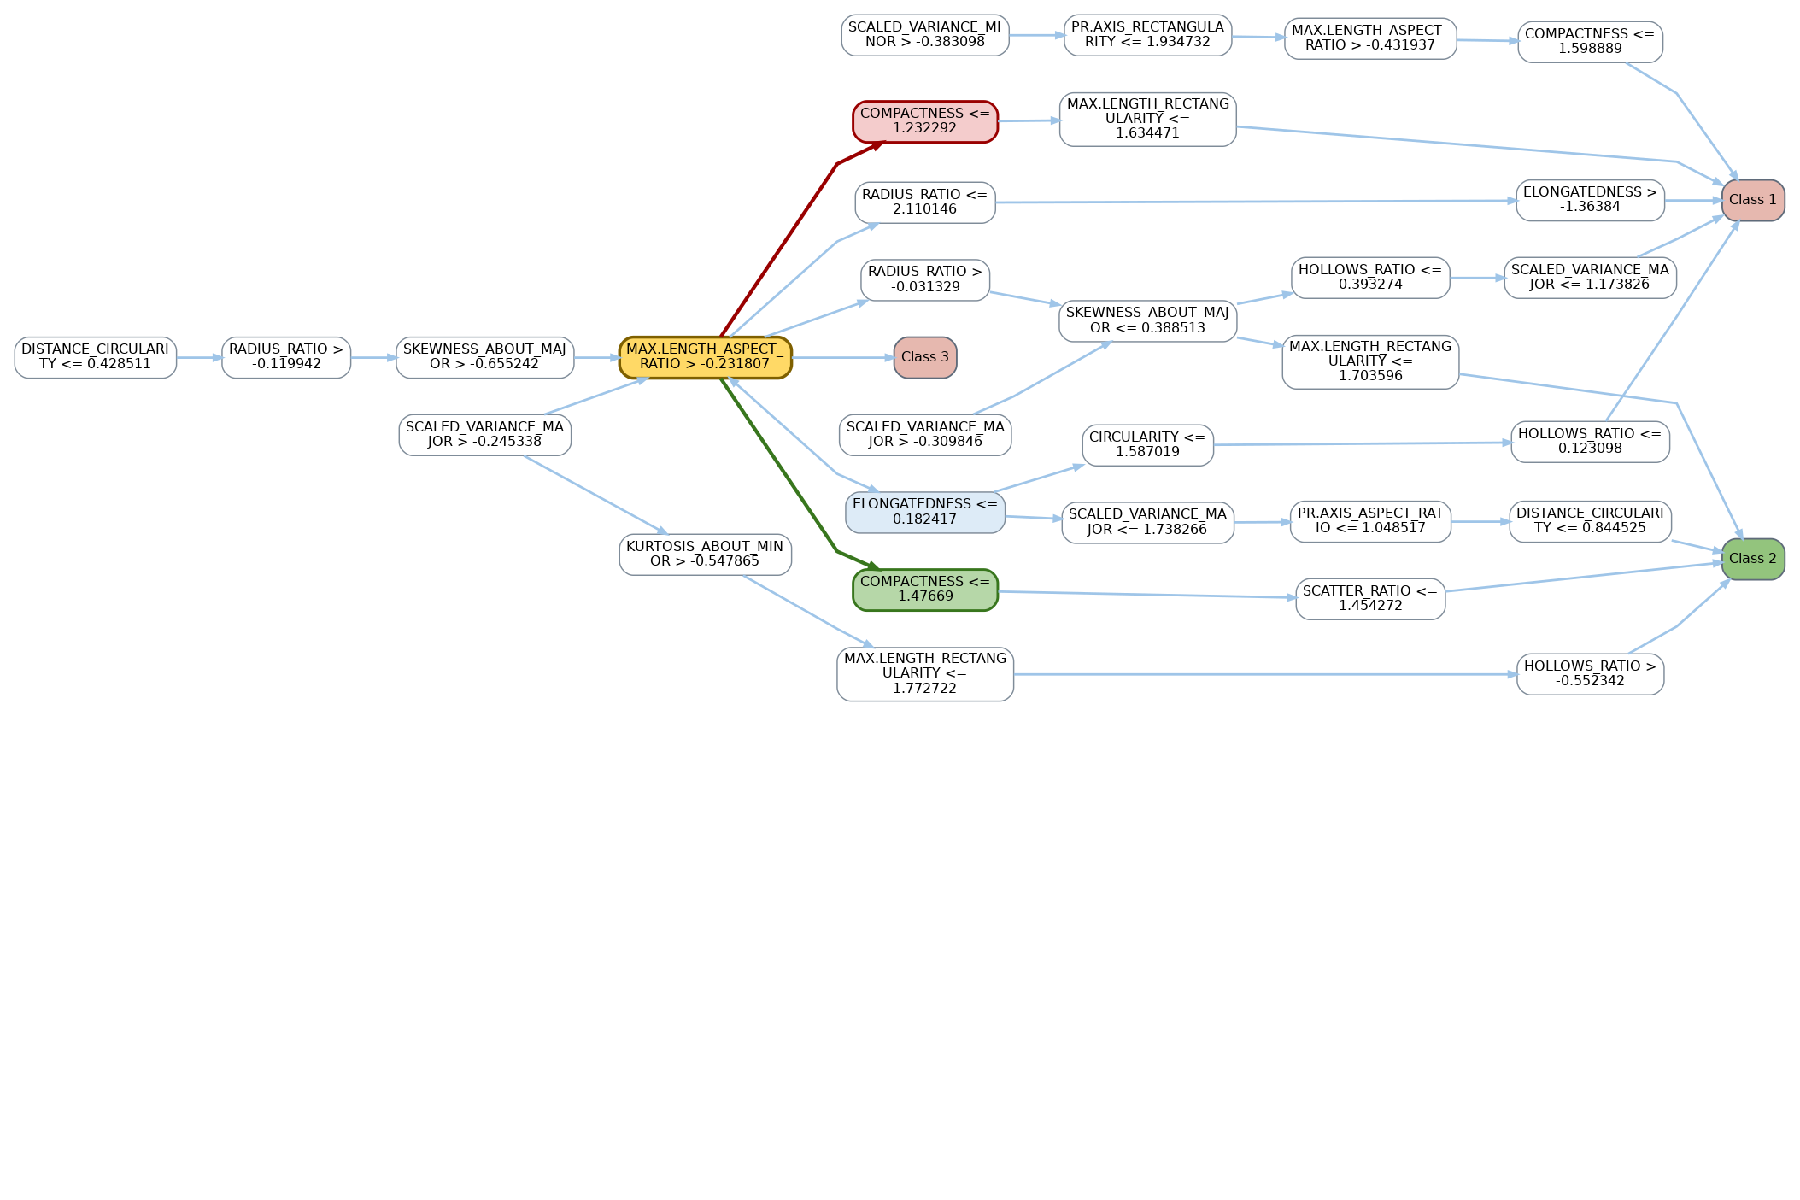
\includegraphics[width=0.99\linewidth,trim={0 8.2cm 0 0},clip]{vehicle_56_execution_trace_aggregate.pdf}
\vspace{1mm} \\
{\tiny
\textbf{Node legend:}
\textcolor{dpgCritical}{$\blacksquare$} critical node\,\,
\textcolor{dpgPredBranch}{$\blacksquare$} predicted branch\,\,
\textcolor{dpgCompBranch}{$\blacksquare$} competitor branch\,\,
%\textcolor{dpgFocus}{$\blacksquare$} focused path\,\,
%\textcolor{dpgContext}{$\blacksquare$} context\,\,
%\textcolor{dpgTrueLeaf}{$\blacktriangle$} true-class leaf\,\,
%\textcolor{dpgOtherLeaf}{$\blacktriangle$} other-class leaf
}
\caption{DPG-local graph for \texttt{vehicle} sample 56 (final
Phase C analysis). The yellow node is the critical node. From this node, the red edge marks the predicted-class successor and the green edge marks the competitor successor. Blue-toned edges represent the remaining local context. thicker edges indicate higher support in the local subgraph.}
\label{fig:phase-cases}
\end{figure}

% -----------------------------------------------------------------------
\section{Discussion}
\label{sec:discussion}
% -----------------------------------------------------------------------

The results show that output-level agreement is an incomplete proxy for explanation quality when the goal is diagnosis rather than justification. Methods such as TreeSHAP, Anchors, and the tree-path baseline are designed to preserve the model output and therefore score strongly on fidelity and local accuracy, whereas DPG-local is designed to preserve the \emph{executed decision structure} and to expose class competition through an explicit local graph. This difference in optimisation targets clarifies how DPG-local should be interpreted in practice: it is not intended to replace attribution-based explanations, but to complement them when analysts need to inspect how a tree ensemble committed to a decision and where plausible alternatives were present. In such workflows, the explanation object matters because a graph of executed predicate transitions can be checked against the model trace and supports questions that are difficult to answer from feature contributions alone---including whether local support is concentrated or contested, where predicted and competitor routes diverge, and if disagreement coincides with a measurable redistribution of support toward alternative classes.

\emph{Structural findings.} The cohort analysis supports this interpretation: disagreement cases are associated with reduced confidence and margin and increased competitor exposure, while trace coverage remains essentially stable, indicating that disagreement reflects a redistribution of local support rather than a failure to recover the executed structure. Because DPG-local edges are formed only from executed traces, edge precision and recombination primarily act as construction-consistency checks, while edge recall and coverage capture whether the extracted local graph retains executed transitions in practice. Evaluation should combine shared output-level metrics with structure-dependent criteria and semantic diagnostics rather than relying on a single fidelity score \cite{nauta2023anecdotal,doshi2017rigorous}.

\emph{Critical nodes and contrastive reasoning.} Critical decision nodes are informative when the strongest predicted and strongest competitor paths share a non-root prefix, and their availability varies across datasets and samples. The current intervention analysis is conservative because it focuses on label flips, whereas probability shifts toward the competitor class can provide a more sensitive signal of diagnostic relevance. Expanding the intervention criterion to soft probability changes would increase the scope of the critical-branch analysis.

\emph{Limitations.} On difficult datasets such as \texttt{isolet} and \texttt{madelon}, lower shared fidelity indicates that DPG-local should be used together with output-aligned explainers when prediction-level agreement is the primary requirement. Scalability is another boundary: although per-sample complexity is linear in executed path length, very deep trees or very large ensembles can substantially increase local graph size and extraction latency, motivating support-threshold pruning strategies for deployment settings. Generalisation beyond majority-vote classification also requires methodological extensions: the current vote-agreement term is defined for hard class votes, so soft-voting or probability-averaging ensembles and regression tasks need alternative agreement terms and, for regression, a revised notion of competitor structure.

\emph{Future directions.} These limitations suggest several lines of future work. User-oriented validation is needed to quantify whether competitor exposure and critical decision gates improve real debugging and auditing decisions beyond what is achievable with feature attribution or rule summaries alone. The confidence score warrants sensitivity analyses of its components and weighting, since the current unweighted formulation is a practical heuristic that could be refined through data-driven calibration. Sufficiency and comprehensiveness evaluations would benefit from conditional perturbation operators that reduce off-manifold effects on correlated features. Finally, extending DPG-local beyond tree ensembles through surrogate models with explicit fidelity controls would broaden the method's applicability to gradient-boosted trees, neural-backed ensembles, and other architectures where path-level tracing remains tractable.


% -----------------------------------------------------------------------
\section{Conclusion}
% -----------------------------------------------------------------------

We proposed DPG-local, an execution-trace formulation of Decision Predicate Graphs for local explanation in tree ensembles, together with a Semantic Graph View providing explanation confidence, competitor exposure, and critical-node diagnostics. The key design principle is that each local graph is built exclusively from the root-to-leaf paths executed by the ensemble for the inspected sample, avoiding the recombination artefacts that arise when transitions are aggregated globally.
Across 15 tabular datasets, DPG-local achieves near-complete transition recovery (edge recall $\approx0.99$) with zero recombination, while edge precision and recombination serve as construction-consistency checks. DPG-local remains competitive on shared output-level metrics against TreeSHAP, LIME, ICE, and Anchors, and the internal DPG-global ablation shows consistent margin improvements (11/15 datasets), confirming that execution-trace construction strengthens competitor separation. The disagreement and cohort analyses further demonstrate that explanation confidence, margin, and competitor exposure jointly characterise prediction/explanation mismatch with large effect sizes, enabling more informative error diagnosis than output agreement alone. These findings position DPG-local as a diagnostic layer for practitioners who need to inspect, audit, or contest tree-ensemble inferences at the path level.

\bibliographystyle{plain}
\bibliography{bibliography}

\end{document}
